
% RECOMMENDED %%%%%%%%%%%%%%%%%%%%%%%%%%%%%%%%%%%%%%%%%%%%%%%%%%%
\documentclass[graybox]{svmult}

% choose options for [] as required from the list
% in the Reference Guide

\usepackage{mathptmx}       % selects Times Roman as basic font
\usepackage{helvet}         % selects Helvetica as sans-serif font
\usepackage{courier}        % selects Courier as typewriter font
\usepackage{type1cm}        % activate if the above 3 fonts are
                            % not available on your system
%
\usepackage{makeidx}         % allows index generation
\usepackage{graphicx}        % standard LaTeX graphics tool
                             % when including figure files
\usepackage{multicol}        % used for the two-column index
\usepackage[bottom]{footmisc}% places footnotes at page bottom

% see the list of further useful packages
% in the Reference Guide

\makeindex             % used for the subject index
                       % please use the style svind.ist with
                       % your makeindex program

%%%%%%%%%%%%%%%%%%%%%%%%%%%%%%%%%%%%%%%%%%%%%%%%%%%%%%%%%%%%%%%%%%%%%%%%%%%%%%%%%%%%%%%%%
\usepackage{multirow}

\begin{document}

\title*{Esquemas de tratamento}
% Use \titlerunning{Short Title} for an abbreviated version of
% your contribution title if the original one is too long
\author{Francisco Hélder Cavalcante Félix e Juvenia Bezerra Fontenele}
% Use \authorrunning{Short Title} for an abbreviated version of
% your contribution title if the original one is too long
\institute{Francisco Hélder Cavalcante Félix \at Centro Pediátrico do Câncer, Hospital Infantil Albert Sabin, R. Alberto Montezuma, 350, 60410-780, Fortaleza - CE \email{fhcflx@outlook.com}
\and Juvenia Bezerra Fontenele \at Faculdade de Farmácia, Odontologia e Enfermagem, Universidade Federal do Ceará, R. Alexandre Baraúna, 949, 60430-160, Fortaleza - CE %\email{juvenia.fontenele@gmail.com}
}
%
% Use the package "url.sty" to avoid
% problems with special characters
% used in your e-mail or web address
%
\maketitle

\abstract{}

\section{Introdução}

No Centro Pediátrico do Câncer do Hospital Infantil Albert Sabin, utilizamos um total de 16 (dezesseis) protocolos de tratamento farmacológico para tumores cerebrais em crianças e adolescentes, baseados na literatura que foi citada neste manual. Estes protocolos foram adaptados a partir dos racionais dos ensaios clínicos descritos, com modificações pertinentes à realidade e disponibilidade de recursos em nosso serviço hospitalar. Além disso, quaisquer conclusões oriundas dos resultados destes ensaios clínicos, bem como informações de outros trabalhos e de outras fontes, foram usadas para adaptar os esquemas de tratamento à luz da melhor evidência disponível no momento em que este manual foi escrito. Alguns dos ensaios clínicos utilizados como modelo para parametrizar nossos protocolos ainda estão em andamento. Neste caso, apenas a parte não randomizada, não experimental dos esquemas foi adaptada e utilizada, mas não os braços de tratamento experimental ou não comprovado por evidências científicas.

\section{O que são estes protocolos}

Protocolo aqui significa um esquema de tratamento baseado em um ensaio clínico patrocinado por grandes grupos cooperativos de tratamento do câncer infantil. Nenhum destes protocolos inclui o texto completo ou trechos dos protocolos originais de pesquisa. Os pacientes tratados em nosso centro seguindo estes protocolos não estão sendo recrutados para pesquisa clínica. Estes protocolos também não constituem diretrizes terapêuticas, nem protocolos clínicos no sentido estrito, pois não foram elaborados por instituições ou grupos organizados, usando metodologia explícita. Nossos protocolos podem ser encarados como rotinas de manuseio dos pacientes e suas patologias, utilizados em nosso serviço hospitalar e baseados em evidências.

Pacientes com condições patológicas que não têm nenhum tratamento amplamente aceito, ou sobre as quais recaem controvérsias quanto à terapêutica, são tratados com  protocolos baseados em evidências preliminares, como ensaios clínicos piloto ou fase I-II, ou ainda revisões de evidências observacionais. Não existem, no momento, ensaios clínicos experimentais abertos em nosso serviço. 

\section{Como utilizar estes protocolos}

Este manuscrito tem fins educativos e é voltado para falantes da língua portuguesa.  Embora este documento seja usado pelo responsável deste projeto como rotina de tratamento dos seus pacientes, o autor não pode responsabilizar-se pelo seu uso em outros locais e para o tratamento de outros pacientes, que não aqueles sob sua estrita supervisão. Os procedimentos e doses de medicamentos descritos no documento são no máximo possível fiéis ao empregado na literatura científica utilizada. No entanto, o autor não pode se responsabilizar por estas doses e seu uso, incluindo o manuseio não criterioso por profissional não habilitado para prescrever e administrar tais medicamentos. 

Apenas médicos registrados de acordo com a legislação vigente em seu país e devidamente habilitados por sociedades de cancerologia (hemato-oncologia) pediátrica devem usar este documento, em parte, ou no todo, e segundo seu juízo, para o tratamento de pacientes. Neste caso, o autor isenta-se de responsabilidade legal sobre quaisquer resultados, incluindo complicações, eventos adversos, prejuízos ou custos, advindos do uso deste documento, ou parte dele, por qualquer outro que não ele mesmo. Ao obter este documento a partir deste projeto, o usuário dele (o documento) está tacitamente concordando com estes e outros termos explicitados aqui.

\section{Declaração ética}

Este manuscrito não necessariamente representa os pontos de vista ou é endossado pelo Hospital Infantil Albert Sabin ou pela Secretaria de Saúde do Estado do Ceará, sendo de iniciativa do responsável pela sua elaboração.

Apesar de tratados conforme os racionais de ensaios clínicos conhecidos, os pacientes não estão sendo recrutados para pesquisa, e isso é deixado claro antes do início do tratamento. Quaisquer esquemas alternativos de tratamento aceitáveis do ponto de vista de chances de sucesso e risco de efeitos adversos são informados aos responsáveis pelos pacientes. Estes podem escolher livremente entre os protocolos propostos ou tratamentos alternativos aceitáveis.

\section{Formato e contribuições}

Nas páginas que se seguem, apresentamos as folhas de acompanhamento ambulatorial dos pacientes que estão em tratamento quimioterápico em nosso serviço hospitalar. Estas folhas são anexadas a cada prontuário do paciente e são preenchidas de acordo com o andamento do tratamento, anotando doses administradas, principais complicações, atrasos, modificações de doses, atualização de informações, entre outros dados. As versões aqui mostradas são as mais atuais quando da publicação deste manual.

O manual foi escrito em LaTeX, usando ShareLatex (depois Overleaf) e programas para desktop (Texmaker). Todo o código do projeto está disponível num repositório público do GitHub, que pode ser acessado neste endereço: 
\begin{quotation}
\texttt{https://github.com/fhcflx/cpc-neuro.git}
\end{quotation}

O arquivo \texttt{*.tex} contém o código correspondente. Contribuições são bem-vindas. Se você ainda não tem uma conta no GitHub (gratuita), inscreva-se, abra uma pendência (\textit{issue}) ou faça uma cópia (\textit{fork}), modifique o que achar necessário e peça para integrar (\textit{pull request}) suas mudanças ao projeto. O sítio do projeto pode ser visitado neste endereço: \texttt{https://fhcflx.github.io/cpc-neuro}. 

\section{Uso não padronizado (\textit{off-label}) de medicamentos}

A definição da ANVISA (Agência Nacional de Vigilância Sanitária) para uso \textit{off-label} de medicamentos é a utilização de um medicamento aprovado para uma determinada indicação em um tratamento não previsto na bula (não aprovado). Isso inclui estudos \textit{a posteriori} que ampliam o uso de um medicamento para outras indicações e também o uso em outras doenças com base em similaridade fisiopatológica. Ainda de acordo com a ANVISA, o "uso \textit{off-label} é, por definição, não autorizado por uma agência reguladora, mas isso não implica que seja incorreto".

Na legislação brasileira atual, não existe regulamentação ou normatização sobre o uso não padronizado de medicamentos. O Conselho Federal de Medicina (CFM), em resposta a um processo-consulta, emitiu o parecer 2/16, no qual define que "os procedimentos médicos \textit{off label} são aqueles em que se utilizam materiais ou fármacos fora das indicações em bula ou protocolos, e sua indicação e prescrição são de responsabilidade do médico. Não compete às Comissões de Ética emitir juízo de valor sobre o uso de \textit{off label}." \cite{cfm}

Para o CFM, o papel das Comissões de Ética Médica e Comitê de Ética em Pesquisa deve ser educativo, uma vez que a responsabilidade do uso não padronizado é toda do médico prescritor. Assim, não há obrigação de reportar o uso não padronizado de medicamentos a nennuma instituição, da mesma forma que não existe exigência de consentimento informado por escrito no território nacional brasileiro para esse uso.

A utilização não padronizada de medicamentos é especialmente frequente na pediatria, uma vez que inexiste incentivo para que empresas que já tem produtos aprovados para adultos arquem com o dispendioso processo de registro da ampliação de seu uso para crianças. \cite{10.1001/archpedi.161.3.282} Uma avaliação mostrou mais de 80\% de prescrições \textit{off-label} em uma UTI neonatal. \cite{CARVALHO2012} Na oncologia pediátrica, existem poucas avaliações semelhantes, mas o uso não padronizado de medicamentos é potencialmente maior ainda. \cite{pmid21453298,10.1111/jcpt.12507}

No caso dos esquemas de tratamento aqui descritos, praticamente todas as medicações têm indicações não padronizadas, seja por faixa etária (etoposido, vincristina, carboplatina, etc) ou por indicação não prevista em bula (vimblastina, cisplatina, ifosfamida e outros). De todas as medicações citadas nesta obra, apenas a ciclofosfamida, a lomustina e a temozolomida (quando usada para tratar gliomas de alto grau) são utilizadas de acordo com a aprovação da ANVISA.

Diversos autores já frisaram a necessidade de mais estudos a fim de validar as indicações, apresentações e vias de administração próprias da pediatria de todas as drogas utilizadas na prática clínica. Uma iniciativa como essa não pode esperar a iniciativa privada, que têm baixa probabilidade de investir em um processo dispendioso e sem retorno financeiro. Seria papel dos governos regular e fomentar o desenvolvimento das aplicações pediátricas de drogas. Infelizmente, em nosso país não existe programa governamental que contemple esse problema.

\section{Avaliação de resposta:}

Não existem critérios de avaliação de resposta criados especificamente para serem utilizados na rotina clínica em pacientes pediátricos com tumores do sistema nervoso central. Os critérios de avaliação de resposta mais amplamente usados baseiam-se nos critérios de resposta da Organização Mundial da saúde (OMS)\cite{10.1093/jnci/92.3.205} e estão listados na tabela abaixo:

\begin{table}[h!]
	\begin{center}
		\begin{tabular}{l|c|c r}
			\multicolumn{2}{l}{\textbf{Resposta}} & \textbf{Método 2D} & \textbf{Método 3D}\\
			\hline
			Resposta completa & RC & Desaparecimento completo & Desaparecimento completo\\
			Resposta parcial & RP & Redução $\geq 50\%$ & Redução $\geq 65\%$ \\
			Resposta menor & RM & Redução $25-50\%$ & Redução $40-65\%$ \\
			Doença estável & DE & Mudança $< 25\%$ & Mudança $< 40\%$ \\
			Progressão & RP & Aumento $\geq 25\%$ & Redução $\geq 40\%$ \\
			\hline
			\multicolumn{4}{l}{\small{2D = bidimensional, 3D = tridimensional}}
		\end{tabular}
	\end{center}
\end{table}

\begin{figure}[h!]
	\begin{center}
		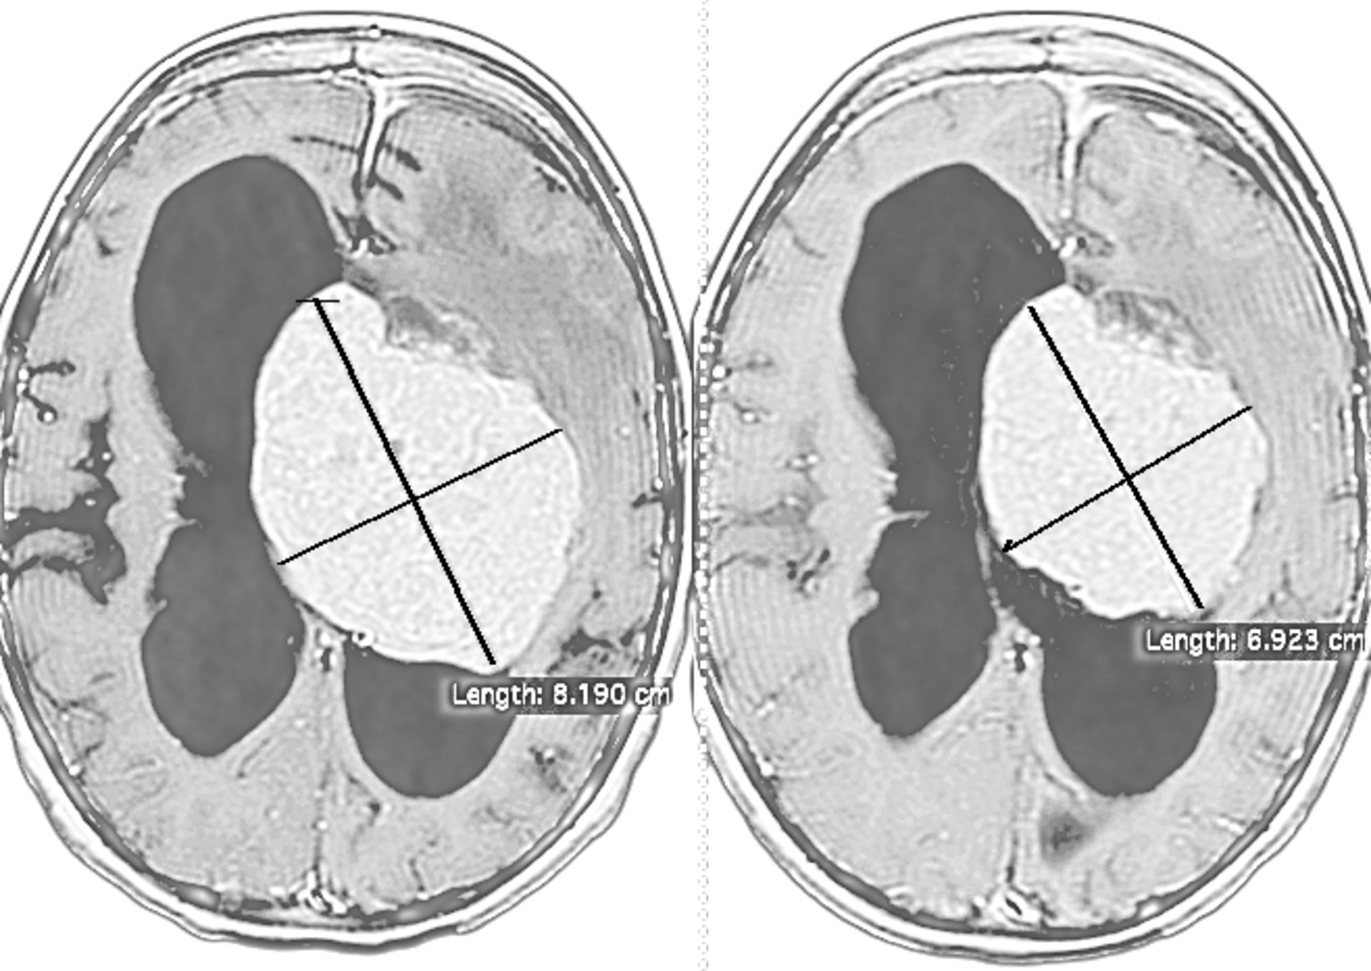
\includegraphics[scale=0.3]{fig/fig6.pdf}
		\caption{Exemplo de medida bidimensional (2D) em dois momentos, mostrando avaliação de resposta. Antes do tratamento, a lesão mediu $8,19 \times 6,2 cm = 50,8$, depois do tratamento, mediu $6,92 \times 5,5 cm = 38,1$. O cálculo da resposta é feito obtendo o produto dos maiores diâmetros perpendiculares e dividindo o valor posterior pelo valor anterior. $R = 38,1 \div 50,8 = 0,75$ Neste caso, ocorreu uma redução objetiva de 25\% pelo método 2D, o que autoriza a classificação da resposta como \textit{menor} (imagem do arquivo do autor, modificada com o programa Gimp 2.8.}
		%\label{Rotulo}
	\end{center}
\end{figure}

A imagem onde a(s) lesão(s) aparece(m) com maior tamanho deve ser escolhida. As medidas subsequentes devem ser realizadas sempre no mesmo plano (axial, sagital, coronal) e aproximadamente mesmo nível da imagem inicial. No exemplo da figura acima, o plano é axial e o nível é logo acima dos núcleos da base. A lesão de grandes proporções ocupa o ventrículo lateral direito e atravessa a linha média. A imagem pós-tratamento é nitidamente menor, mas essa redução precisa ser objetivamente quantificada. Escolhendo-se a imagem com maior área lesional no corte axial, mede-se os dois maiores diâmetros perpendiculares entre si. O produto destes diâmetros é uma estimativa do volume tumoral (método 2D). O método 2D tem maior acurácia na pediatria \cite{warren}.

A comparação entre os valores antes e após o tratamento mostra que ocorreu uma redução de 25\% do valor estimado para o tamanho tumoral. Esta magnitude de redução encontra-se no limite entre a ausência de mudança (doença estável) e uma mudança menos significativa (resposta menor), ilustrando como a inspeção visual e a avaliação quantitativa podem dar impressões subjetivas diferentes. A avaliação quantitativa da resposta é imprescindível para classificar adequadamente os pacientes e decidir a conduta clínica.


\bibliographystyle{unsrt}
\bibliography{cpc-neuro2014/bib}

\end{document}
